\section{Experiments}\label{foi.exp}
In this section, we describe several experiments (methods and results) to %SM: consider indicating number of experiments as can help reader with expectatons... 
highlight differences among the various approaches %SM: various approaches that have been previously used yes?
to modelling HIV transmission via sexual partnerships.
Specifically:
\sref{foi.exp.xph}~and~\ref{foi.exp.dur} examine how
the calculated per-partnership probability of transmission $B$ differs under assumptions of:
within- \vs between-partnership heterogeneity in the per-act probability of transmission $\beta$,
and 1-year \vs complete partnership durations $\delta$; then
\sref{foi.exp.model} explores differences in key transmission model outputs
among the force of infection equations from \sref{foi.prior}~and~\ref{foi.prop}.
In many transmission models,
a justification for chosing each specific approach is rarely given. %SM: could cite your review paper or Rao paper?
Thus, to support future use and justification for selecting a given aproach, this section aims to illustrate potential implications of these choices.  %SM: in many ways an implication of your work is to support/inform rationale for model selection :) - i think that is what you were trying to tell me when we discussed the conclusion of the abstract!
%===================================================================================================
\subsection{Within- \vs Between-Partnership Heterogeneity}\label{foi.exp.xph}
For computing an average per-partnership probability of transmission $B$,
\sref{foi.prior.xph} clarified the interpretations of
\eqref{eq:B.wph} \vs \eqref{eq:B.bph} as modelling
within-partnership heterogeneity (WPH) \vs between-partnership heterogeneity (BPH), respectively.
As shown in \sref{sr.foi.proof}, $B_{\wph} \ge B_{\bph}$.
Here we explore under what conditions the ratio $B_{\wph}~/~B_{\bph}$ is maximized
--- \ie when does the choice of approach matter most.
For simplicity, we considered a single illustrative factor
affecting $\alpha \in [0,1]$ proportion of sex acts ($1-\alpha$ are unaffected),
with relative probability of transmission $R \in [0.01,10]$.
We then computed $B_{\wph}$ and $B_{\bph}$ for $A \in [1,1000]$ total sex acts,
using a base per-act probability of transmission $\beta = 0.34$\%
as a representative value for HIV \cite{Boily2009}.
\par
\begin{figure}
  \centering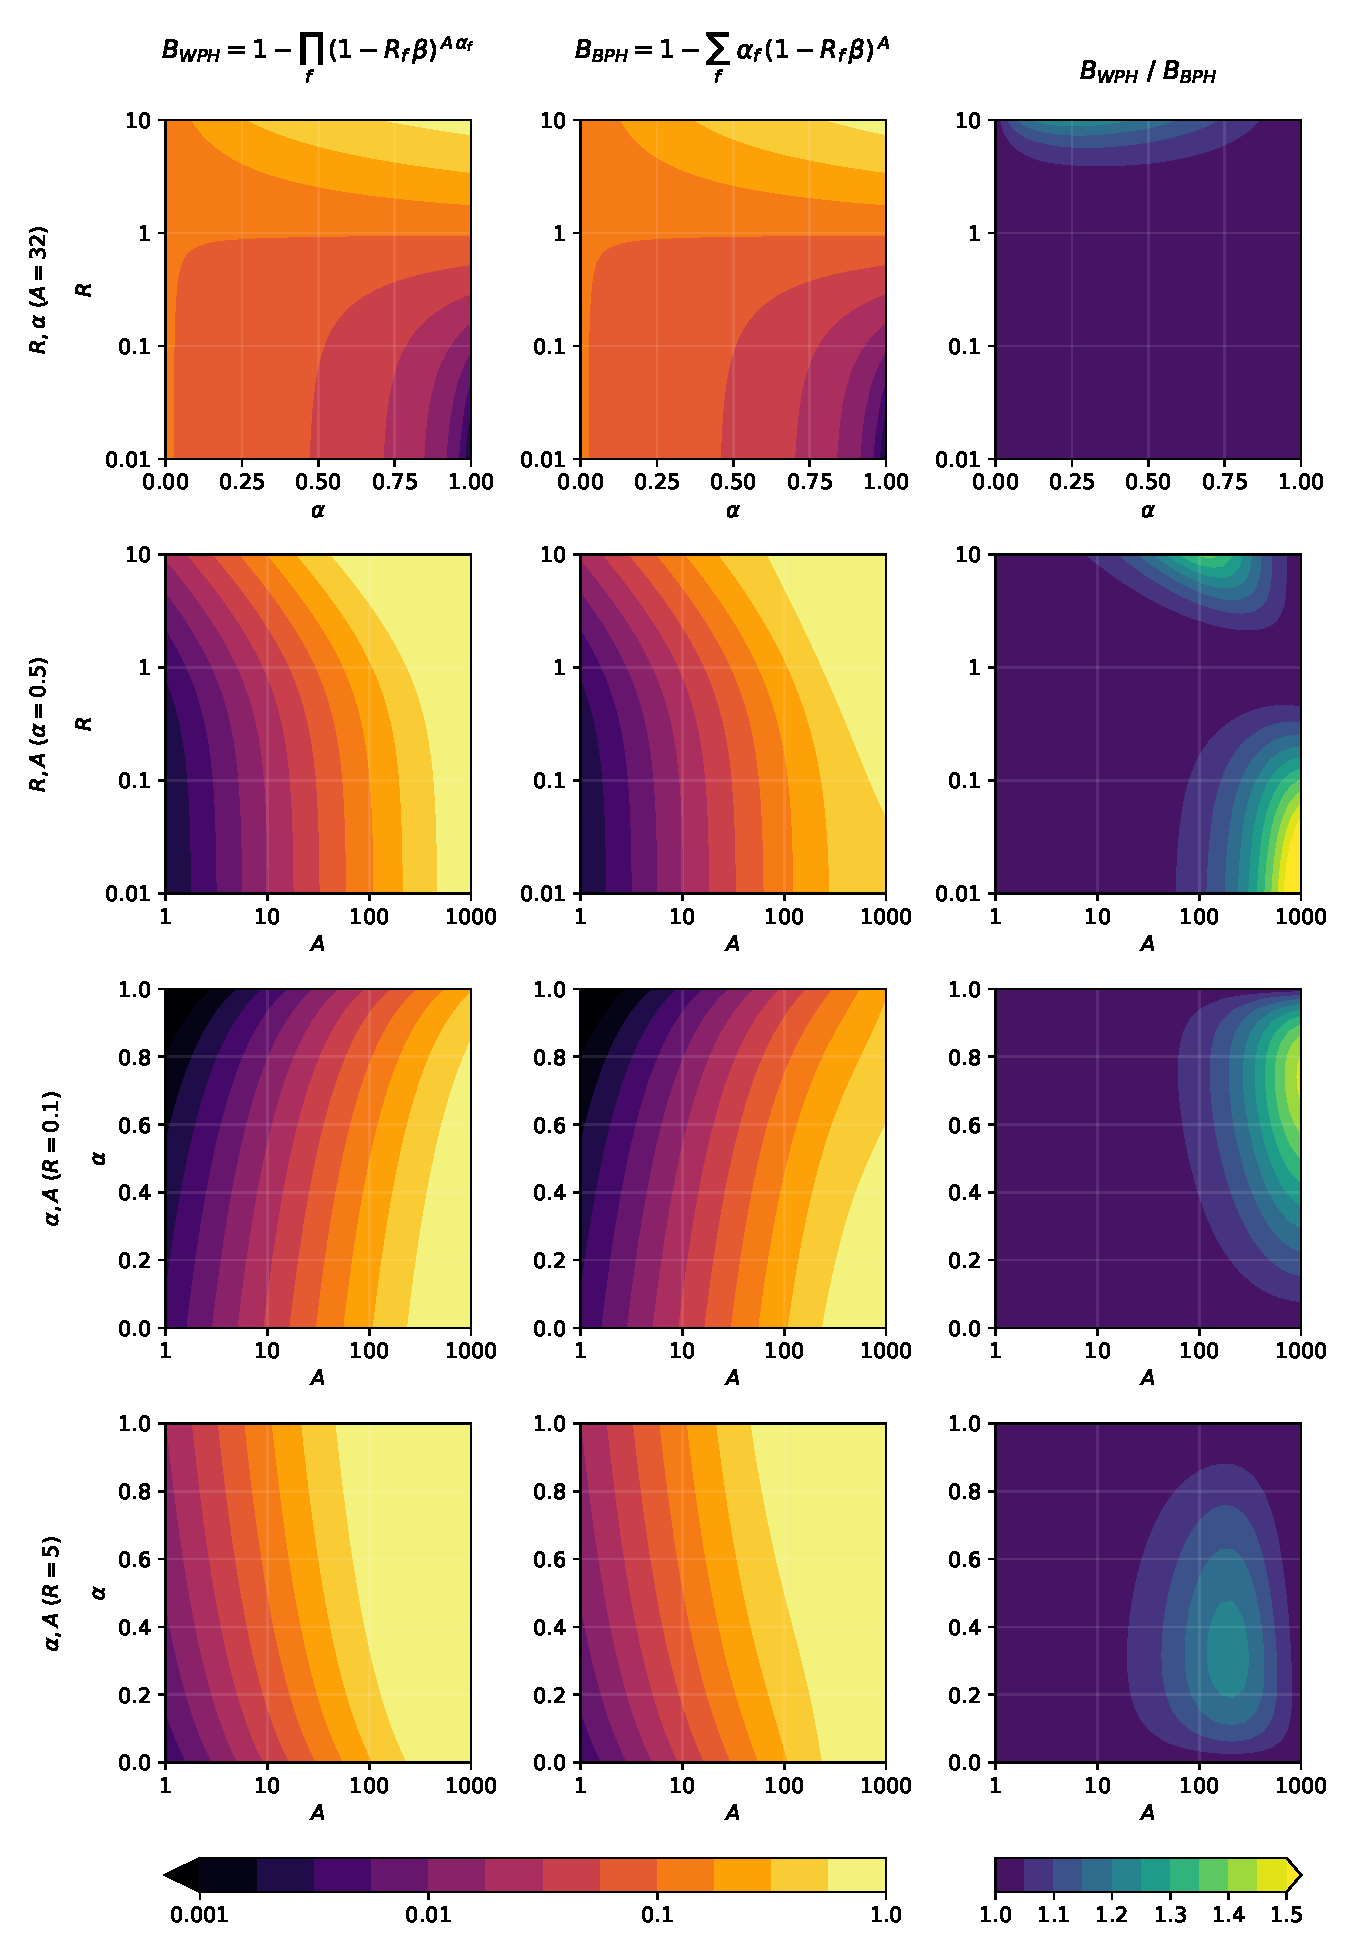
\includegraphics[scale=.6]{B.xph.surf}
  \caption{Average per-partnership probability of transmission $B$
    given heterogeneity in the per-act probability of transmission $\beta$
    within \vs between partnerships}
  \label{fig:B.xph.surf}
  \floatfoot{
    $B$: probability of transmission per partnership (log scale colourmap);
    $\beta = 0.34\%$: base probability of transmission per sex act (fixed) \cite{Boily2009};
    $A$: total sex acts per partnership (log scale);
    $\alpha$: proportion of sex acts affected by factor (linear scale);
    $R$: relative $\beta$ given factor (log scale);
    WPH: within-partnership heterogeneity;
    BPH: between-partnership heterogeneity.}
\end{figure}
\begin{figure}
  \centering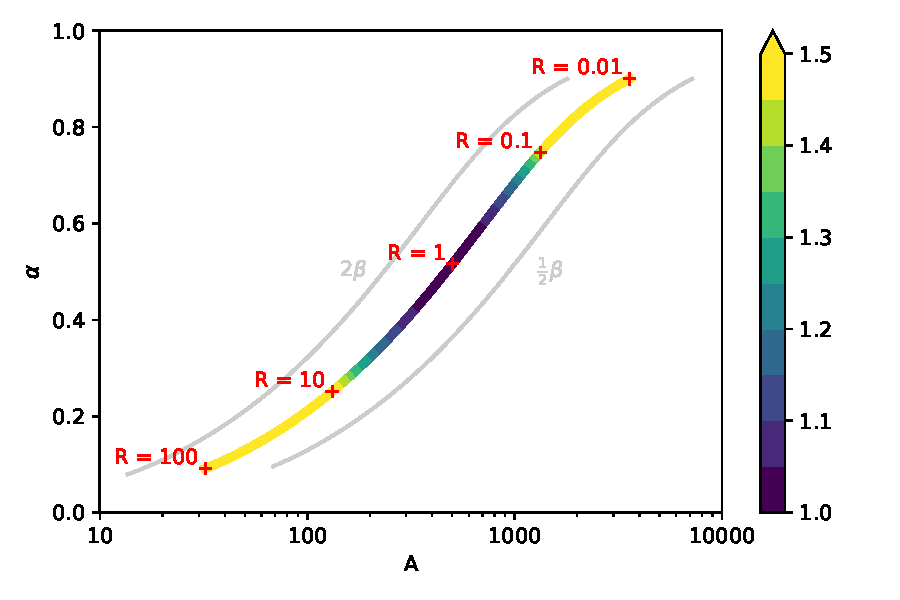
\includegraphics[scale=.6]{B.xph.max}
  \caption{Parameter values $(\alpha,A)$ which maximize the difference between
    the average per-partnership probability of transmission
    given within- \vs between-partnership heterogeneity}
  \label{fig:B.xph.max}
  \floatfoot{
    $B_{\wph}~/~B_{\bph}$: line colour;
    $\beta = 0.34\%$: probability of transmission per sex act (fixed) \cite{Boily2009};
    $A$: total sex acts per partnership (log scale);
    $\alpha$: proportion of sex acts affected by factor (linear scale);
    $R$: relative $\beta$ given factor (log scale);
    gray lines denote equivalent contours for $2\beta$~and~$\frac12\beta$.}
\end{figure}
Figure~\ref{fig:B.xph.surf} illustrates four 2-dimensional cross sections of $B(R,\alpha,A)$
under WPH \vs BPH, and the ratio $B_{\wph} / B_{\bph}$;
the cross sections were at: $A = 32$, $\alpha = 0.5$, $R = 0.1$, and $R = 5$.
Based on these results, the difference between approaches can be summarized as:
negligible for $A < 10$, and small for $A < 100$;
increasing as $R$ gets farther from 1 ($R \rightarrow 0$ or $R \rightarrow \infty$); and
maximized by specific values of $(\alpha,A)$ for a given $R$, including
$\alpha > \frac12$ for $R < 1$, and $\alpha < \frac12$ for $R > 1$.
The specific values of $(\alpha,A)$ which maximize
the difference between approaches for a given $R$ and $\beta$
create a continuous curve (Figure~\ref{fig:B.xph.max}), which slowly tends towards
$\alpha \rightarrow 1, A \rightarrow \infty$ as $R \rightarrow 0$, and
$\alpha \rightarrow 0, A \rightarrow 0$ as $R \rightarrow \infty$.
The curve is sigmoidal for log-transformed $A$,
and shifts left with increasing $\beta$.
We did not derive an analytical expression, but it should be possible to do so.
In the context of HIV, the difference between approaches would be
larger for protective factors (\eg condoms)
affecting most of a large number of sex acts ($\alpha > 1000$);
and likewise larger for risk-increasing factors (\eg anal sex)
affecting a minority of a moderate number of sex acts ($\alpha \approx 100$).
%===================================================================================================
\subsection{Partnership Durations}\label{foi.exp.dur}
As described in \sref{foi.prior.ptr}, multiple prior models have
implicitly assumed a maximum partnership duration $\delta \le 1$ year.
As such, the adjustment for inert sex acts \eqref{eq:B} would have reduced effect.
This reduction can be quantified via
the effective probability of transmission per sex act $\beta'$
--- \ie tangent slopes in Figure~\ref{fig:binom.dur} --- defined as:
\begin{equation}\label{eq:beta.eff}
  \beta' = \frac{B}{A} = \frac{1 - {(1 - \beta)}^{A}}{A}
\end{equation}
Figure~\ref{fig:dur.surf} illustrates
the 1-year $\beta'_1$ \vs true-duration $\beta'_\delta$, for different
partnership durations $\delta \in [1, 30]$ year and
sex frequencies $F \in [1,180]$ per year.
Assuming $\delta \le 1$ can considerably increase the modelled rate of transmission
for partnerships with $F \ge 52$ (\ie weekly) and a true duration $\delta \ge 5$ years,
including up to \emph{8-fold} difference with
$F \approx 100$ per year and $\delta \approx 30$ years.
This suggests that prior models using $\delta \le 1$ could have
substantially overestimated the relative contribution of
longer partnerships with frequent sex --- including main/spousal partnerships ---
to overall transmission, as further evidenced below in \sref{foi.exp.model}.
\begin{figure}
  \centering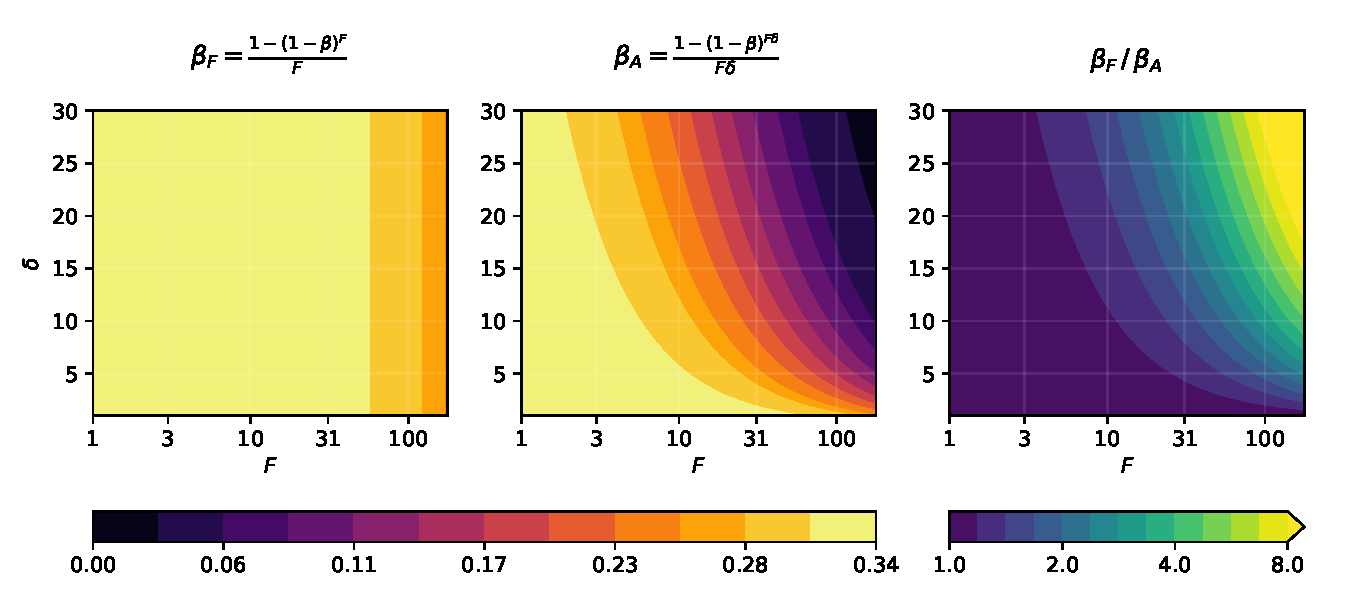
\includegraphics[scale=.6]{dur.surf}
  \caption{Effective probability of transmission per sex act
    over 1 year \vs total partnership duration}
  \label{fig:dur.surf}
  \floatfoot{
    $\beta = 0.34\%$: probability of transmission per sex act (fixed) \cite{Boily2009};
    $F$: frequency of sex per partnership (per year, log scale);
    $\delta$: partnership duration (years, linear scale);
    $\beta_1, \beta_\delta$: effective probability of transmission per sex act,
      for 1 year \vs total partnership duration, respectively.}
\end{figure}
%===================================================================================================
\subsection{Comparing Approaches in a Transmission Model}\label{foi.exp.model}
Next, we sought to explore how different approaches to
modelling and parameterizing the force of infection equation
influence key outputs from a full transmission model.
We focused on two aspects of prior approaches:
whether or not partnership durations are effectively capped at 1 year (\sref{foi.prior.dur}), and
whether incidence is aggregated across partnerships as a rate \vs proportion (\sref{foi.prior.ptr}).
Thus, we considered 3 prior approaches:
\emph{Instantaneous Rate-Duration}~(\ird),
\emph{Instantaneous Rate-1-Year}~(\iry), and
\emph{Instantaneous Proportion-1-Year}~(\ipy),
plus the \emph{Effective Partnerships Adjustment} (\epa) approach
proposed in \sref{foi.prop}
(Table~\ref{tab:foi.models}).
Among these 4 approaches, we sought to characterize (aims):
\begin{enumerate}
  \item \label{obj:foi.dyn}
  fundamental differences in transmission dynamics under each approach
  \item \label{obj:foi.tpaf}
  differences in model-estimated prevention priorities under each approach
  \end{enumerate}
For aim~\ref{obj:foi.dyn}, we compared group-specific HIV incidence
using \emph{equal} model parameters across approaches.
While the specific parameters required by each approach are slightly different,
we derived these parameters from a consistent set of ``upstream'' parameters as described below.
For aim~\ref{obj:foi.tpaf}, we compared selected
transmission population attributable fractions (TPAFs, details below)
using \emph{approach-specific} (\ie recalibrated) model parameters.
Since applied models are usually calibrated to a given context,
aim~\ref{obj:foi.tpaf} thus provides a realistic comparison of
how prevention priorities could differ when informed by distinct models using each approach.
\begin{table}
  \centering
  \caption{Compared approaches to modelling HIV transmission via sexual partnerships}
  \label{tab:foi.models}
  \begin{tabular}{clcl}
  \toprule
  ID & Name & Key Eqs. & Key Parameters \\
  \midrule
  \ird & \emph{Instantaneous Rate-Duration}       & (\ref{eq:B.bph}),~(\ref{eq:foi.ir}) & $A,Q$        \\
  \iry & \emph{Instantaneous Rate-1-Year}         & (\ref{eq:B.bph}),~(\ref{eq:foi.ir}) & $A_1,Q_1$    \\
  \ipy & \emph{Instantaneous Proportion-1-Year}   & (\ref{eq:B.bph}),~(\ref{eq:foi.ip}) & $A_1,Q_1$    \\
  \epa & \emph{Effective Partnerships Adjustment} & (\ref{eq:M.SI})--(\ref{eq:foi.jh})  & $K,F,\delta$ \\
  \bottomrule
\end{tabular}
\floatfoot{
  $K$: number of concurrent partners;
  $F$: frequency of sex per partnership;
  $\delta$: partnership duration;
  $A = F\delta$: total sex acts per partnership;
  $Q = K/\delta$: partnership formation rate;
  $A_1 = F \delta_1$, $Q_1 = K/\delta_1$, where $\delta_1 = \min{(\delta,1)}$.}

\end{table}
%---------------------------------------------------------------------------------------------------
\paragraph{Eswatini HIV Transmission Model}
We integrated each approach within an existing compartmental model
of heterosexual HIV transmission in Eswatini \cite{Knight2024art}
(full details in Appendix~\ref{mod}).
Briefly, the model includes: 2~sexes, 4~levels of sexual activity
(including female sex workers [FSW] and their clients)
and 4 partnership types (Figure~\ref{fig:model.risk}): % MAN below
main/spousal (14--19 years long, lowest condom use),
casual (3--18 months, moderate condom use),
one-off sex work (1 sex act, highest condom use), and
repeat sex work (2--12 months, high condom use).
The model also includes
5 stages of HIV infection (Figure~\ref{fig:model.hiv}) and
5 stages of the HIV treatment cascade (Figure~\ref{fig:model.cascade}), plus
anal \vs vaginal sex, male circumcision, and genital ulcer disease,
with differences over time and/or risk groups.
%---------------------------------------------------------------------------------------------------
\paragraph{Equal \& Approach-Specific Parameters}
We calibrated the model separately under each approach
using an adapted version of Incremental Mixture Importance Sampling (IMIS) \cite{Raftery2010}
(full details in \sref{mod.cal})
yielding 1000 model fits (parameter sets) per approach.
For all approaches, we directly specified or sampled the following ``upstream parameters'':
mean numbers of reported partners $x$ per person for a given recall period ($\omega$:
12 months for main/spousal and casual; 1 month for one-off and repeat sex work;
details in \sref{mod.par.pnum}),
partnership durations $\delta$ (see \sref{mod.par.pdur}), and
sex frequencies per partnership $F$ (see \sref{mod.par.fsex}).
Then, we derived the required ``downstream parameters'' for each approach
--- \ie $K$, $F$, and $\delta$ for \epa; $Q$ and $A$ for \ird, \iry, and \ipy\ ---
as shown in Figure~\ref{fig:diag.foi.par}.
For aim~\ref{obj:foi.dyn} we used \emph{equal} upstream parameters from \epa model fits,
while for aim~\ref{obj:foi.dyn} we used \emph{approach-specific} parameters.
\par
Appendix~\ref{sr.cal} provides detailed results of model calibration under the \epa approach.
Appendix~\ref{sr.foi.cal} provides selected results of model calibration under all 4 approaches,
including Figures~\ref{fig:fit.prev.foi}--\ref{fig:fit.inc1v2.foi} which illustrate
model-estimated HIV prevalence, incidence, and ratios thereof
\vs calibration targets under each approach.
Model fits under each approach were qualitatively similar,
though overall log-likelihoods were highest under \ipy and lowest under \iry % MAN
(Figure~\ref{fig:ll.hist.foi}).
Most posterior parameter distributions also differed significantly among approaches
(rank score test \cite{Kruskal1952}, Figure~\ref{fig:post.distr.foi}).
% TODO: (*) try to summarize patterns / trends in differences?
\begin{figure}
  \centering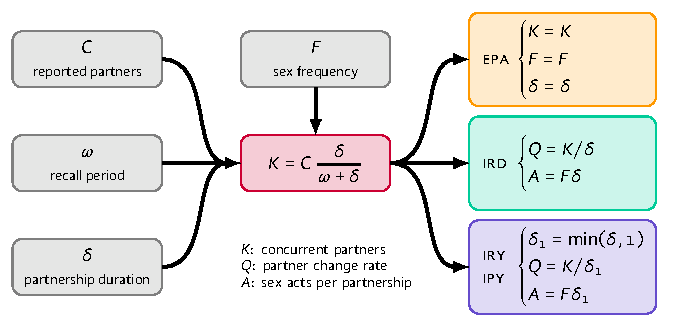
\includegraphics[scale=1]{diag.foi.par}
  \caption{Flow chart for deriving model parameters for each force of infection approach
    from a consistent set of upstream parameters}
  \label{fig:diag.foi.par}
  \floatfoot{\fffoi. See \cite{Knight2023bias} for $K$ equation.}
\end{figure}
%---------------------------------------------------------------------------------------------------
\paragraph{Transmission-Driven Seroconcordance}
Figure~\ref{fig:fit.tdsc.foi} illustrates the modelled
transmission-driven seroconcordance (TDSC) proportion for each partnership type
among infected individuals --- \ie using denominator (b) from \sref{foi.prop.tdsc}.
This model output is only possible under the \epa approach, and reflects
the relative reduction in onward transmission risk among infected individuals
due to infections ``trapped'' within partnerships.
The TDSC proportion increases rapidly for all partnership types during epidemic growth,
but later declines alongside HIV incidence.
% TODO: (?) % TDSC is related to: incidence (convolve) ptr duration distribution
The TDSC proportion tends to be higher for
longer partnerships (\eg main/spousal \vs other types) and for
partnership types with lower concurrency (\eg casual \vs sex work).
Since the TDSC proportion varies across time, partnership types, and risk groups,
it may be challenging to define a simplified incidence adjustment
to account for trapped infections in existing transmission models.
\begin{figure}
  \centering\includegraphics[scale=\fitscale]{fit.tdsc.base.all}
  \caption{Modelled transmission-driven seroconcordance within different partnership types}
  \label{fig:fit.tdsc.foi}
  \floatfoot{\fffit; \ffribbon.}
\end{figure}
%---------------------------------------------------------------------------------------------------
\subsubsection{Transmission Dynamics using Equal Parameters}\label{foi.exp.mod.dyn}
Figure~\ref{fig:foi.ep.incidence} illustrates HIV incidence among
FSW, clients, and everybody else (``lower risk'')
under each approach using equal parameters.
Specifically, Figure~\ref{fig:foi.ep.incidence.raw} illustrates incidence per person-year
(\epa repeated across panels for comparison)
and Figure~\ref{fig:foi.ep.incidence.rel} illustrates relative differences \vs the \epa approach.%
\footnote{Relative differences were ``paired'' according to each parameter set $k$,
  and computed as $(\textsc{ixx}_k - \epa_k) / \epa_k$.}
We made the following observations and hypothesized explanations.
\par
First, incidence among lower risk groups
was generally much higher under 1-year approaches (\iry,~\ipy).
Underestimation of inert sex acts under these approaches
disproportionately increases transmission via main/spousal partnerships,
allowing more transmission to/from lower risk individuals,
including a positive feedback loop via
increasing HIV prevalence among lower risk individuals
given like-with-like mixing (see \sref{mod.par.mix.odds}).
Second, incidence differences between
the 1-year approaches (\iry,~\ipy) \vs \epa generally grew over time.
The \epa approach explicitly models the accumulation of
transmission-driven seroconcordant partnerships (Figure~\ref{fig:fit.tdsc})
wherein all sex acts are inert.
Thus, by underestimating inert sex acts throughout the epidemic,
the 1-year approaches are initially less biased \vs \epa, but later overestimate incidence.
Third, incidence among FSW and clients was lower under the ``incidence proportion'' approach (\ipy).
Incidence proportion \eqref{eq:foi.ip} treats all transmission risks as competing,
and notably forces incidence $\lambda^\ip \le 1$,
disproportionately reducing incidence among those at highest risk.
Finally, incidence under the full-duration approach (\ird) was consistently similar to \epa.
Complete accounting of inert sex acts under this approach
effectively delays transmission in longer partnership types,
but with limited impact on overall dynamics because
shorter partnerships contribute the majority of new infections,
especially during epidemic growth.
% TODO: (*) why does ird > epa before 1990: instant onward transmission risk?
\begin{figure}
  \subcapoverlap
  \foreach \var in {raw,rel}{
  \begin{subfigure}{\linewidth}
    \centering
    \includegraphics[width=.975\linewidth]{foi.ep.incidence.\var}
    \caption{\raggedright}
    \label{fig:foi.ep.incidence.\var}
  \end{subfigure}}
  \caption{HIV incidence among selected risk groups,
    estimated under different prior force of infection approaches (colours)
    \vs the \emph{Effective Partnerships Adjustment} approach using equal model parameters}
  \label{fig:foi.ep.incidence}
  \floatfoot{\fffoi;
    \sfref{fig:foi.ep.incidence.raw} absolute incidence;
    \sfref{fig:foi.ep.incidence.rel} relative differences: $(\textsc{ixx}_k - \epa_k) / \epa_k$;
    \ffpopz; \ffribbon.}
\end{figure}
\par
Figure~\ref{fig:foi.wiw.ptr} further illustrates the proportions of modelled yearly HIV infections
transmitted via different partnership types under each approach
using equal parameters (top) and approach-specific parameters for comparison (bottom).
For equal parameters, the 1-year approaches (\iry,~\ipy) featured
the greatest proportions of transmission via main/spousal partnerships, and the least via sex work.
By contrast, the full-duration approach (\ird) featured
the smallest proportions transmitted via main/spousal partnerships, and the most via sex work.
The distribution under \epa was in between these two extremes,
but overall closer to \ird.
%---------------------------------------------------------------------------------------------------
\subsubsection{Prevention Priorities using Approach-Specific Parameters}\label{foi.exp.mod.tpaf}
Many models applied to assess HIV prevention priorities model specific intervention scenarios.
However, these context-specific intervention details
require additional analyses and/or assumptions,
and only explore a subset of the modelled transmission pathways.
By contrast, the TPAF reflects an ``intervention agnostic'' measure of
how any given transmission pathway contributes to transmission overall.
TPAFs are an extension of classic PAFs which additionally capture
the downstream infections averted by preventing upstream infections \cite{Mishra2014tpaf}.
The TPAF among population $j$ of transmission pathway $k$ is defined as
the relative difference in cumulative infections $\Omega$ among $j$ since a given time $t_0$
with \vs without transmission via $k$:
\begin{equation}\label{eq:tpaf}
  \textup{TPAF}_{jk}(t) = \frac{\Omega_{j}(t) - \Omega_{jk} (t)}{\Omega_{j}(t)}
  ,\qquad
  \Omega_{jk}(t) = \int_{t_0}^{t} \Lambda_{j,M_k=0}(\tau)\,d\tau
  ,\qquad
  t = t_0 + \Delta_t
\end{equation}
Thus, TPAFs reflect hypothetical interventions with perfect prevention,
ignoring practical implementation challenges associated with any real intervention.
Like classic PAFs, TPAFs can sum to more than 100\% \cite{Rowe2004,Mishra2021}.
\par
We computed TPAFs among the population overall ($j$)
for 6 transmission pathways ($k$):
transmission from FSW, clients, and everybody else (``lower risk''); and
transmission via main/spousal, casual, and sex work (one-off and repeat combined) partnership types.
% JK: @SM we originally had 1,3,10 year time horizons
%     However, the TPAFs and differences across approaches were so similar across time horizons
%     I decided to remove the horizon stratification altogether and just use 3-year horizons
%     and then combine the figure for risk groups and partnership types.
%     This also prompted me to add 2020 (was previously 1990-2010)
%     where we see FSW/client/SW TPAFs all bounce back up
We computed 3-year TPAFs for each pathway
after recalibration under each of the 4 force of infection approaches,
starting in $t_0 = {}$1990, 2000, 2010, and 2020 (96 total TPAFs).
We implemented scenarios without transmission via a given pathway
using a boolean ``mask'' applied to the mixing matrix $M_{pii'}$,
\emph{after} resolving the values per \sref{mod.par.mix},
such that mixing patterns were not affected.
\par
\begin{figure}
  \includegraphics[width=\linewidth]{foi.tpaf.3x2}
  \caption{3-Year TPAFs of transmission
    from different risk groups (top row) and
    via different partnership types (bottom row)
    starting from different $t_0$ (x-axis),
    estimated under different force of infection approaches (colours)}
  \label{fig:foi.tpaf}
  \floatfoot{\fffoi; \fftpaf; \ffbox.}
\end{figure}
Figure~\ref{fig:foi.tpaf} illustrates the 3-year TPAFs
for the 6 transmission pathways explored.
Trends in TPAFs across risk groups and approaches
were similar for 1- and 10-year time horizons (results not shown).
As $t_0$ increased from 1990 through 2010, TPAFs generally
decreased for FSW, clients, and sex work overall, and
increased for lower risk groups, main/spousal and casual partnerships;
these trends then reversed in 2020.
Such trends are consistent with prior work showing that
TPAFs of key populations are typically large at first,
decrease in widespread HIV epidemics, and
are anticipated to increase again as incidence declines
\cite{Johnson2011,Mishra2012sr,Boily2015,Brown2019,Garnett2021}.
\par
Differences in TPAFs across force of infection approaches were
largest for main/spousal partnerships, with TPAFs
under the 1-year approaches (\iry,~\ipy) significantly larger than
under the full-duration approach (\ird).
Main/spousal TPAFs under \epa were similar to \iry~and~\ipy in 1990,
but tended closer to \ird from 2000 onward.
These trends reflect that fact that only \epa captures
a growing proportion of inert sex acts over time,
whereas \iry~and~\ipy effectively estimate a small static proportion,
while \ird estimates a large static proportion.
Relative differences across approaches in lower risk population TPAFs were
similar (but less pronounced) to main/spousal partnership TPAFs, while
casual partnership and client population TPAFs were
opposite (but also less pronounced);
TPAFs for FSW and sex work overall were similar across approaches.
\par
In general, we observed TPAF differences across approaches
in the absence of pathway-specific calibration targets.
For example, model recalibration under each approach to
HIV incidence and prevalence targets for FSW (\sref{mod.cal.targ})
induced compensatory shifts in posterior parameter distributions
(Figure~\ref{fig:post.distr.foi})
which counteracted the innate differences in
transmission via sex work under each approach.
By contrast, none of the available calibration targets directly inform
the relative contribution of main/spousal \vs casual partnerships to overall transmission
(and our model parameterization allows all risk groups to form both types),
so innate differences between approaches directly shape differences in TPAFs.
Similarly, we assumed that calibration targets for
men reporting 2+ sexual partners in the past 12 months
reflected a mixture of clients and non-clients
(Tables~\ref{tab:targ.prev}--\ref{tab:targ.ir}),
hence persistent TPAF differences for lower risk and client populations as well.
% TODO: (*) Figure~\ref{fig:wiw.base.alluvial}
